\section{Java Sample applications}
\label{sec:JavaSampleApps}

The first two examples in this section are simple applications developed in COMPSs to easily illustrate how to code,
compile and run COMPSs applications. These applications are executed locally and show different ways to take advantage
of all the COMPSs features. 

The rest of the examples are more elaborated and consider the execution in a cloud platform where the VMs mount a common 
storage on \textbf{/sharedDisk} directory. This is useful in the case of applications that require working 
with big files, allowing to transfer data only once, at the beginning of the execution, and to enable 
the application to access the data directly during the rest of the execution.

The Virtual Machine available at our webpage (\url{http://compss.bsc.es/}) provides a development environment with
all the applications listed in the following sections. The codes of all the applications can be found under the 
$/home/compss/tutorial\_apps/java/$ folder. 

%%%%%%%%%%%%%%%
%% HELLO WORLD 
%%%%%%%%%%%%%%%
\subsection{Hello World}
The Hello Wolrd is a Java application that creates a task and prints a Hello World! message. Its purpose is to clarify that the 
COMPSs tasks output is redirected to the job files and it is \textbf{not} available at the standard output. 

Next we provide the important parts of the application's code.

\begin{lstlisting}[language=java]
	// hello.Hello
	
	public static void main(String[] args) throws Exception {
		// Check and get parameters
		if (args.length != 0) {
			usage();
			throw new Exception("[ERROR] Incorrect number of parameters");
		}
		
		// Hello World from main application
		System.out.println("Hello World! (from main application)");

		// Hello World from a task
		HelloImpl.sayHello();
	}
\end{lstlisting}

As shown in the main code, this application has no input arguments. 

\begin{lstlisting}[language=java]
	// hello.HelloImpl
	
	public static void sayHello() {
		System.out.println("Hello World! (from a task)");
	}
\end{lstlisting}

Remember that, to run with COMPSs, java applications must provide an interface. For simplicity, in this example, the content of the interface only
declares the task which has no parameters:

\begin{lstlisting}[language=java]
	// hello.HelloItf
	
	@Method(declaringClass = "hello.HelloImpl")
	void sayHello(
	);
\end{lstlisting}

Notice that there is a first Hello World message printed from the main code and, a second one, printed inside a task. When executing sequentially
this application users will be able to see both messages at the standard output. However, when executing this application with COMPSs, users will only
see the message from the main code at the standard output. The message printed from the task will be stored inside the job log files. 

Let's try it. First we proceed to compile the code by running the following instructions:

\begin{lstlisting}[language=bash]
compss@bsc:~$ cd ~/tutorial_apps/java/hello/src/main/java/hello/
compss@bsc:~/tutorial_apps/java/hello/src/main/java/hello$ javac *.java
compss@bsc:~/tutorial_apps/java/hello/src/main/java/hello$ cd ..
compss@bsc:~/tutorial_apps/java/hello/src/main/java$ jar cf hello.jar hello
compss@bsc:~/tutorial_apps/java/hello/src/main/java$ mv hello.jar ~/tutorial_apps/java/hello/jar/
\end{lstlisting}

Alternatively, this example application is prepared to be compiled with \textit{maven}:

\begin{lstlisting}[language=bash]
compss@bsc:~$ cd ~/tutorial_apps/java/hello/
compss@bsc:~/tutorial_apps/java/hello$ mvn clean package
\end{lstlisting}

Once done, we can sequentially execute the application by directly invoking the \textit{jar} file.

\begin{lstlisting}[language=bash]
compss@bsc:~$ cd ~/tutorial_apps/java/hello/jar/
compss@bsc:~/tutorial_apps/java/hello/jar$ java -cp hello.jar hello.Hello 
Hello World! (from main application)
Hello World! (from a task)
\end{lstlisting}

And we can also execute the application with COMPSs:

\begin{lstlisting}[language=bash]
compss@bsc:~$ cd ~/tutorial_apps/java/hello/jar/
compss@bsc:~/tutorial_apps/java/hello/jar$ runcompss -d hello.Hello
[  INFO] Using default execution type: compss
[  INFO] Using default location for project file: /opt/COMPSs/Runtime/configuration/xml/projects/default_project.xml
[  INFO] Using default location for resources file: /opt/COMPSs/Runtime/configuration/xml/resources/default_resources.xml

----------------- Executing hello.Hello --------------------------

WARNING: COMPSs Properties file is null. Setting default values
[(928)    API]  -  Deploying COMPSs Runtime v<version>
[(931)    API]  -  Starting COMPSs Runtime v<version>
[(931)    API]  -  Initializing components
[(1472)    API]  -  Ready to process tasks
Hello World! (from main application)
[(1474)    API]  -  Creating task from method sayHello in hello.HelloImpl
[(1474)    API]  -  There is 0 parameter
[(1477)    API]  -  No more tasks for app 1
[(4029)    API]  -  Getting Result Files 1
[(4030)    API]  -  Stop IT reached
[(4030)    API]  -  Stopping AP...
[(4031)    API]  -  Stopping TD...
[(4161)    API]  -  Stopping Comm...
[(4163)    API]  -  Runtime stopped
[(4166)    API]  -  Execution Finished

------------------------------------------------------------
\end{lstlisting}

Notice that the COMPSs execution is using the \textit{-d} option to allow the job logging. Thus, we can check out the application jobs folder to look for
the task output.

\begin{lstlisting}[language=bash]
compss@bsc:~$ cd ~/.COMPSs/hello.Hello_01/jobs/
compss@bsc:~/.COMPSs/hello.Hello_01/jobs$ ls -1
job1_NEW.err
job1_NEW.out
compss@bsc:~/.COMPSs/hello.Hello_01/jobs$ cat job1_NEW.out
[JAVA EXECUTOR] executeTask - Begin task execution
WORKER - Parameters of execution:
  * Method type: METHOD
  * Method definition: [DECLARING CLASS=hello.HelloImpl, METHOD NAME=sayHello]
  * Parameter types:
  * Parameter values:
Hello World! (from a task)
[JAVA EXECUTOR] executeTask - End task execution
\end{lstlisting}

%%%%%%%%%%%%%%%
%% SIMPLE
%%%%%%%%%%%%%%%
\subsection{Simple}
The Simple application is a Java application that increases a counter by means of a task. The counter is stored inside a file that 
is transferred to the worker when the task is executed. Thus, the tasks inferface is defined as follows:

\begin{lstlisting}[language=java]
	// simple.SimpleItf
	
	@Method(declaringClass = "simple.SimpleImpl")
	void increment(
		@Parameter(type = Type.FILE, direction = Direction.INOUT) String file
	);
\end{lstlisting}

Next we also provide the invocation of the task from the main code and the increment's method code.

\begin{lstlisting}[language=java]
	// simple.Simple
	
	public static void main(String[] args) throws Exception {
		// Check and get parameters
		if (args.length != 1) {
			usage();
			throw new Exception("[ERROR] Incorrect number of parameters");
		}
		int initialValue = Integer.parseInt(args[0]);

		// Write value
		FileOutputStream fos = new FileOutputStream(fileName);
		fos.write(initialValue);
		fos.close();
		System.out.println("Initial counter value is " + initialValue);

		//Execute increment
		SimpleImpl.increment(fileName);

		// Write new value
		FileInputStream fis = new FileInputStream(fileName);
		int finalValue = fis.read();
		fis.close();
		System.out.println("Final counter value is " + finalValue);
	}
\end{lstlisting}

\begin{lstlisting}[language=java]
	// simple.SimpleImpl
	
	public static void increment(String counterFile) throws FileNotFoundException, IOException {
		// Read value
		FileInputStream fis = new FileInputStream(counterFile);
		int count = fis.read();
		fis.close();
		
		// Write new value
		FileOutputStream fos = new FileOutputStream(counterFile);
		fos.write(++count);
		fos.close();
	}
\end{lstlisting}

Finally, to compile and execute this application users must run the following commands:

\begin{lstlisting}[language=bash]
compss@bsc:~$ cd ~/tutorial_apps/java/simple/src/main/java/simple/
compss@bsc:~/tutorial_apps/java/simple/src/main/java/simple$ javac *.java
compss@bsc:~/tutorial_apps/java/simple/src/main/java/simple$ cd ..
compss@bsc:~/tutorial_apps/java/simple/src/main/java$ jar cf simple.jar simple
compss@bsc:~/tutorial_apps/java/simple/src/main/java$ mv simple.jar ~/tutorial_apps/java/simple/jar/

compss@bsc:~$ cd ~/tutorial_apps/java/simple/jar
compss@bsc:~/tutorial_apps/java/simple/jar$ runcompss simple.Simple 1
compss@bsc:~/tutorial_apps/java/simple/jar$ runcompss simple.Simple 1
[  INFO] Using default execution type: compss
[  INFO] Using default location for project file: /opt/COMPSs/Runtime/configuration/xml/projects/default_project.xml
[  INFO] Using default location for resources file: /opt/COMPSs/Runtime/configuration/xml/resources/default_resources.xml

----------------- Executing simple.Simple --------------------------

WARNING: COMPSs Properties file is null. Setting default values
[(772)    API]  -  Starting COMPSs Runtime v<version>
Initial counter value is 1
Final counter value is 2
[(3813)    API]  -  Execution Finished

------------------------------------------------------------
\end{lstlisting}


%%%%%%%%%%%%%%%
%% Increment
%%%%%%%%%%%%%%%
\subsection{Increment}
The Increment application is a Java application that increases N times three different counters. Each increase step is developed by a separated task. The
purpose of this application is to show parallelism between the three counters.

Next we provide the main code of this application. The code inside the \textit{increment} task is the same than the previous example. 

\begin{lstlisting}[language=java]
	// increment.Increment
	public static void main(String[] args) throws Exception {
		// Check and get parameters
		if (args.length != 4) {
			usage();
			throw new Exception("[ERROR] Incorrect number of parameters");
		}
		int N = Integer.parseInt(args[0]);
		int counter1 = Integer.parseInt(args[1]);
		int counter2 = Integer.parseInt(args[2]);
		int counter3 = Integer.parseInt(args[3]);
		
		// Initialize counter files
		System.out.println("Initial counter values:");
		initializeCounters(counter1, counter2, counter3);
		
		// Print initial counters state
		printCounterValues();

		// Execute increment tasks
		for (int i = 0; i < N; ++i) {
			IncrementImpl.increment(fileName1);
			IncrementImpl.increment(fileName2);
			IncrementImpl.increment(fileName3);
		}

		// Print final counters state (sync)
		System.out.println("Final counter values:");
		printCounterValues();
	}
\end{lstlisting}

As shown in the main code, this application has 4 parameters that stand for:

\begin{enumerate}
 \item \textbf{N:} Number of times to increase a counter
 \item \textbf{InitialValue1:} Initial value for counter 1
 \item \textbf{InitialValue2:} Initial value for counter 2
 \item \textbf{InitialValue3:} Initial value for counter 3
\end{enumerate}

Next we will compile and run the Increment application with the \textit{-g} option to be able to generate the final graph at the end of the execution.

\begin{lstlisting}[language=bash]
compss@bsc:~$ cd ~/tutorial_apps/java/increment/src/main/java/increment/
compss@bsc:~/tutorial_apps/java/increment/src/main/java/increment$ javac *.java
compss@bsc:~/tutorial_apps/java/increment/src/main/java/increment$ cd ..
compss@bsc:~/tutorial_apps/java/increment/src/main/java$ jar cf increment.jar increment
compss@bsc:~/tutorial_apps/java/increment/src/main/java$ mv increment.jar ~/tutorial_apps/java/increment/jar/

compss@bsc:~$ cd ~/tutorial_apps/java/increment/jar
compss@bsc:~/tutorial_apps/java/increment/jar$ runcompss -g increment.Increment 10 1 2 3
[  INFO] Using default execution type: compss
[  INFO] Using default location for project file: /opt/COMPSs/Runtime/configuration/xml/projects/default_project.xml
[  INFO] Using default location for resources file: /opt/COMPSs/Runtime/configuration/xml/resources/default_resources.xml

----------------- Executing increment.Increment --------------------------

WARNING: COMPSs Properties file is null. Setting default values
[(1028)    API]  -  Starting COMPSs Runtime v<version>
Initial counter values:
- Counter1 value is 1
- Counter2 value is 2
- Counter3 value is 3
Final counter values:
- Counter1 value is 11
- Counter2 value is 12
- Counter3 value is 13
[(4403)    API]  -  Execution Finished

------------------------------------------------------------
\end{lstlisting}

By running the \textit{compss\_gengraph} command users can obtain the task graph of the above execution. Next we provide the set of commands to obtain the
graph show in Figure \ref{fig:increment_java}.

\begin{lstlisting}[language=bash]
compss@bsc:~$ cd ~/.COMPSs/increment.Increment_01/monitor/
compss@bsc:~/.COMPSs/increment.Increment_01/monitor$ compss_gengraph complete_graph.dot
compss@bsc:~/.COMPSs/increment.Increment_01/monitor$ evince complete_graph.pdf
\end{lstlisting}

\begin{figure}[ht!]
  \centering
    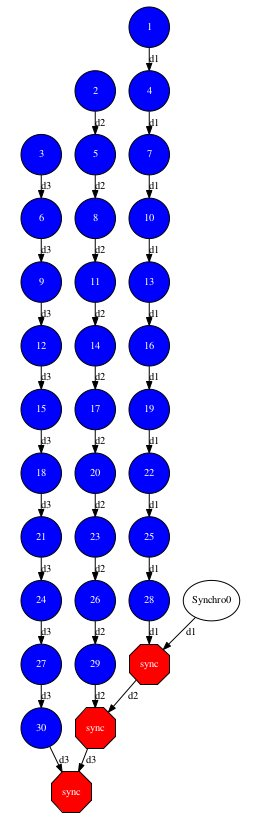
\includegraphics[width=0.3\textwidth]{./Sections/2_Java/Figures/increment_graph.jpeg}
    \caption{Java increment tasks graph} 
    \label{fig:increment_java}
\end{figure}

%%%%%%%%%%%%%%%
%% MATMUL
%%%%%%%%%%%%%%%
\newpage
\subsection{Matrix multiplication}
The Matrix Multiplication (Matmul) is a pure Java application that multiplies two matrices in a direct way. 
The application creates 2 matrices of N x N size initialized with values, and multiply the matrices by blocks.

This application provides three different implementations that only differ on the way of storing the matrix:
\begin{enumerate}
 \item \textbf{matmul.objects.Matmul} Matrix stored by means of objects
 \item \textbf{matmul.files.Matmul} Matrix stored in files
 \item \textbf{matmul.arrays.Matmul} Matrix represented by an array
\end{enumerate}

\begin{figure}[ht!]
  \centering
    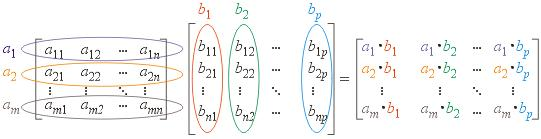
\includegraphics[width=0.8\textwidth]{./Sections/2_Java/Figures/matrix.jpeg}
    \caption{Matrix multiplication} 
    \label{fig:matrix}
\end{figure}

\newpage 
In all the implementations the multiplication is implemented in the multiplyAccumulative method that is thus selected as the task to be executed remotely.
As example, we we provide next the task implementation and the tasks interface for the objects implementation.

\begin{lstlisting}[language=java]
	// matmul.objects.Block
	public void multiplyAccumulative(Block a, Block b) {
		for (int i = 0; i < M; i++) {
			for (int j = 0; j < M; j++) {
				for (int k = 0; k < M; k++) {
					data[i][j] += a.data[i][k]*b.data[k][j];
				}
			}
		}
	}
\end{lstlisting}

\begin{lstlisting}[language=java]
	// matmul.objects.MatmulItf
	@Method(declaringClass = "matmul.objects.Block")
	void multiplyAccumulative(
		@Parameter Block a,
		@Parameter Block b
	);
\end{lstlisting}

In order to run the application the matrix dimension (number of blocks) and the dimension of each block have to be supplied. Consequently, any of the 
implementations must be executed by running the following command.
\begin{lstlisting}[language=bash]
compss@bsc:~$ runcompss matmul.<IMPLEMENTATION_TYPE>.Matmul <matrix_dim> <block_dim>
\end{lstlisting}

Finally, we provide an example of execution for each implementation.

\begin{lstlisting}[language=bash]
compss@bsc:~$ cd ~/tutorial_apps/java/matmul/jar/
compss@bsc:~/tutorial_apps/java/matmul/jar$ runcompss matmul.objects.Matmul 8 4
[  INFO] Using default execution type: compss
[  INFO] Using default location for project file: /opt/COMPSs/Runtime/configuration/xml/projects/default_project.xml
[  INFO] Using default location for resources file: /opt/COMPSs/Runtime/configuration/xml/resources/default_resources.xml

----------------- Executing matmul.objects.Matmul --------------------------

WARNING: COMPSs Properties file is null. Setting default values
[(887)    API]  -  Starting COMPSs Runtime v<version>
[LOG] MSIZE parameter value = 8
[LOG] BSIZE parameter value = 4
[LOG] Allocating A/B/C matrix space
[LOG] Computing Result
[LOG] Main program finished.
[(7415)    API]  -  Execution Finished

------------------------------------------------------------
\end{lstlisting}

\begin{lstlisting}[language=bash]
compss@bsc:~$ cd ~/tutorial_apps/java/matmul/jar/
compss@bsc:~/tutorial_apps/java/matmul/jar$ runcompss matmul.files.Matmul 8 4
[  INFO] Using default execution type: compss
[  INFO] Using default location for project file: /opt/COMPSs/Runtime/configuration/xml/projects/default_project.xml
[  INFO] Using default location for resources file: /opt/COMPSs/Runtime/configuration/xml/resources/default_resources.xml

----------------- Executing matmul.files.Matmul --------------------------

WARNING: COMPSs Properties file is null. Setting default values
[(907)    API]  -  Starting COMPSs Runtime v<version>
[LOG] MSIZE parameter value = 8
[LOG] BSIZE parameter value = 4
[LOG] Computing result
[LOG] Main program finished.
[(9925)    API]  -  Execution Finished

------------------------------------------------------------
\end{lstlisting}


\begin{lstlisting}[language=bash]
compss@bsc:~$ cd ~/tutorial_apps/java/matmul/jar/
compss@bsc:~/tutorial_apps/java/matmul/jar$ runcompss matmul.arrays.Matmul 8 4
[  INFO] Using default execution type: compss
[  INFO] Using default location for project file: /opt/COMPSs/Runtime/configuration/xml/projects/default_project.xml
[  INFO] Using default location for resources file: /opt/COMPSs/Runtime/configuration/xml/resources/default_resources.xml

----------------- Executing matmul.arrays.Matmul --------------------------

WARNING: COMPSs Properties file is null. Setting default values
[(1062)    API]  -  Starting COMPSs Runtime v<version>
[LOG] MSIZE parameter value = 8
[LOG] BSIZE parameter value = 4
[LOG] Allocating C matrix space
[LOG] Computing Result
[LOG] Main program finished.
[(7811)    API]  -  Execution Finished

------------------------------------------------------------
\end{lstlisting}


%%%%%%%%%%%%%%%
%% SPARSELU 
%%%%%%%%%%%%%%%
\subsection{Sparse LU decomposition}
SparseLU multiplies two matrices using the factorization method of LU decomposition, which factorizes a 
matrix as a product of a lower triangular matrix and an upper one.

\begin{figure}[ht!]
  \centering
    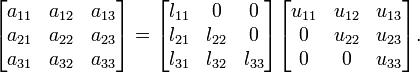
\includegraphics[width=0.6\textwidth]{./Sections/2_Java/Figures/SparseLU.jpeg}
    \caption{Sparse LU decomposition}
    \label{fig:SparseLO}
\end{figure}

The matrix is divided into N x N blocks on where 4 types of operations will be applied modifying the blocks: 
{\bf lu0}, {\bf fwd}, {\bf bdiv} and {\bf bmod}. These four operations are implemented in four methods that 
are selecetd as the tasks that will be executed remotely. In order to run the application the matrix dimension 
has to be provided.

As the previous application, the sparseLU is provided in three different implementations that only differ on the way of storing
the matrix:
\begin{enumerate}
 \item \textbf{sparseLU.objects.SparseLU} Matrix stored by means of objects
 \item \textbf{sparseLU.files.SparseLU} Matrix stored in files
 \item \textbf{sparseLU.arrays.SparseLU} Matrix represented by an array
\end{enumerate}

Thus, the commands needed to execute the application is with each implementation are:

\begin{lstlisting}[language=bash]
compss@bsc:~$ cd tutorial_apps/java/sparseLU/jar/
compss@bsc:~/tutorial_apps/java/sparseLU/jar$ runcompss sparseLU.objects.SparseLU 16 8
[  INFO] Using default execution type: compss
[  INFO] Using default location for project file: /opt/COMPSs/Runtime/configuration/xml/projects/default_project.xml
[  INFO] Using default location for resources file: /opt/COMPSs/Runtime/configuration/xml/resources/default_resources.xml

----------------- Executing sparseLU.objects.SparseLU --------------------------

WARNING: COMPSs Properties file is null. Setting default values
[(1221)    API]  -  Starting COMPSs Runtime v<version>
[LOG] Running with the following parameters:
[LOG]  - Matrix Size: 16
[LOG]  - Block Size:  8
[LOG] Initializing Matrix
[LOG] Computing SparseLU algorithm on A
[LOG] Main program finished.
[(13642)    API]  -  Execution Finished

------------------------------------------------------------
\end{lstlisting}

\begin{lstlisting}[language=bash]
compss@bsc:~$ cd tutorial_apps/java/sparseLU/jar/
compss@bsc:~/tutorial_apps/java/sparseLU/jar$ runcompss sparseLU.files.SparseLU 4 8
[  INFO] Using default execution type: compss
[  INFO] Using default location for project file: /opt/COMPSs/Runtime/configuration/xml/projects/default_project.xml
[  INFO] Using default location for resources file: /opt/COMPSs/Runtime/configuration/xml/resources/default_resources.xml

----------------- Executing sparseLU.files.SparseLU --------------------------

WARNING: COMPSs Properties file is null. Setting default values
[(1082)    API]  -  Starting COMPSs Runtime v<version>
[LOG] Running with the following parameters:
[LOG]  - Matrix Size: 16
[LOG]  - Block Size:  8
[LOG] Initializing Matrix
[LOG] Computing SparseLU algorithm on A
[LOG] Main program finished.
[(13605)    API]  -  Execution Finished

------------------------------------------------------------

\end{lstlisting}

\begin{lstlisting}[language=bash]
compss@bsc:~$ cd tutorial_apps/java/sparseLU/jar/
compss@bsc:~/tutorial_apps/java/sparseLU/jar$ runcompss sparseLU.arrays.SparseLU 8 8
[  INFO] Using default execution type: compss
[  INFO] Using default location for project file: /opt/COMPSs/Runtime/configuration/xml/projects/default_project.xml
[  INFO] Using default location for resources file: /opt/COMPSs/Runtime/configuration/xml/resources/default_resources.xml

----------------- Executing sparseLU.arrays.SparseLU --------------------------

WARNING: COMPSs Properties file is null. Setting default values
[(1082)    API]  -  Starting COMPSs Runtime v<version>
[LOG] Running with the following parameters:
[LOG]  - Matrix Size: 16
[LOG]  - Block Size:  8
[LOG] Initializing Matrix
[LOG] Computing SparseLU algorithm on A
[LOG] Main program finished.
[(13605)    API]  -  Execution Finished

------------------------------------------------------------

\end{lstlisting}


%%%%%%%%%%%%%%%
%% KMEANS
%%%%%%%%%%%%%%%
%\subsection{KMeans}


%%%%%%%%%%%%%%%
%% BLAST
%%%%%%%%%%%%%%%
\subsection{BLAST Workflow}
BLAST is a widely-used bioinformatics tool for comparing primary biological sequence information, such as 
the amino-acid sequences of different proteins or the nucleotides of DNA sequences with sequence databases, 
identifying sequences that resemble the query sequence above a certain threshold. 
The work performed by the COMPSs Blast workflow is computationally intensive and embarrassingly parallel.

\begin{figure}[ht!]
  \centering
    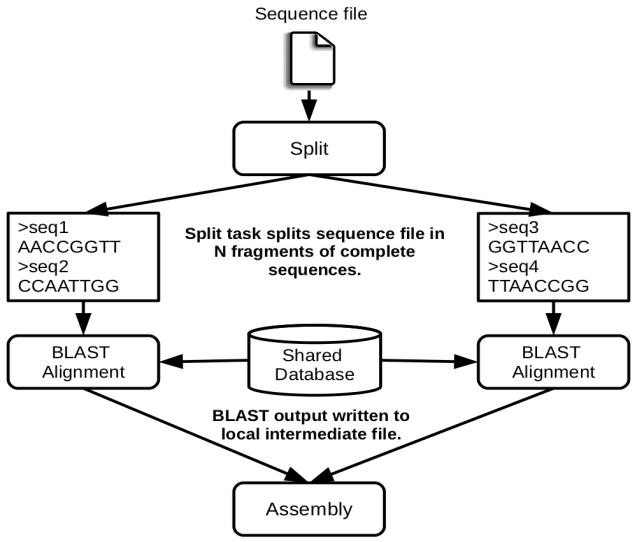
\includegraphics[width=0.7\textwidth]{./Sections/2_Java/Figures/blast_workflow.jpeg}
    \caption{The COMPSs Blast workflow}
    \label{fig:BLAST_workflow}
\end{figure}

The workflow describes the three blocks of the workflow implemented in the {\bf Split}, {\bf Align} and 
{\bf Assembly} methods. The second one is the only method that is chosen to be executed remotely, so it 
is the unique method defined in the interface file. The {\bf Split} method chops the query sequences file 
in N fragments, {\bf Align} compares each sequence fragment against the database by means of the Blast 
binary, and {\bf Assembly} combines all intermediate files into a single result file.

This application uses a database that will be on the shared disk space avoiding transferring the entire 
database (which can be large) between the virtual machines.

\begin{lstlisting}[language=bash]
compss@bsc:~$ cp ~/workspace/blast/package/Blast.tar.gz /home/compss/
compss@bsc:~$ tar xzf Blast.tar.gz
\end{lstlisting}

The command line to execute the workflow:

\begin{lstlisting}[language=bash]
compss@bsc:~$ runcompss blast.Blast <debug> 
                                    <bin_location>
                                    <database_file> 
                                    <sequences_file>
                                    <frag_number> 
                                    <tmpdir>
                                    <output_file>
\end{lstlisting}

Where:
\begin{itemize}
 \item {\bf debug}: The debug flag of the application (true or false).
 \item {\bf bin\_location}: Path of the Blast binary.
 \item {\bf database\_file}: Path of database file; the shared disk {\bf /sharedDisk/} is suggested to avoid big data transfers.
 \item {\bf sequences\_file}: Path of sequences file.
 \item {\bf frag\_number}: Number of fragments of the original sequence file, this number determines the number of parallel Align tasks.
 \item {\bf tmpdir}: Temporary directory ({\bf /home/compss/tmp/}).
 \item {\bf output\_file}: Path of the result file.
\end{itemize}
 
Example:
\begin{lstlisting}[language=bash]
compss@bsc:~$ runcompss blast.Blast true
                        /home/compss/tutorial_apps/java/blast/binary/blastall
                        /sharedDisk/Blast/databases/swissprot/swissprot
                        /sharedDisk/Blast/sequences/sargasso_test.fasta 
                        4 
                        /tmp/
                        /home/compss/out.txt
\end{lstlisting}